\section{Rancangan Solusi}
\label{sec:rancangan-solusi}

Langkah umum untuk mencapai solusi masalah di Tugas Akhir ditunjukkan pada gambar \ref*{fig:langkah-umum} berikut.

\begin{figure}[ht]
    \centering
    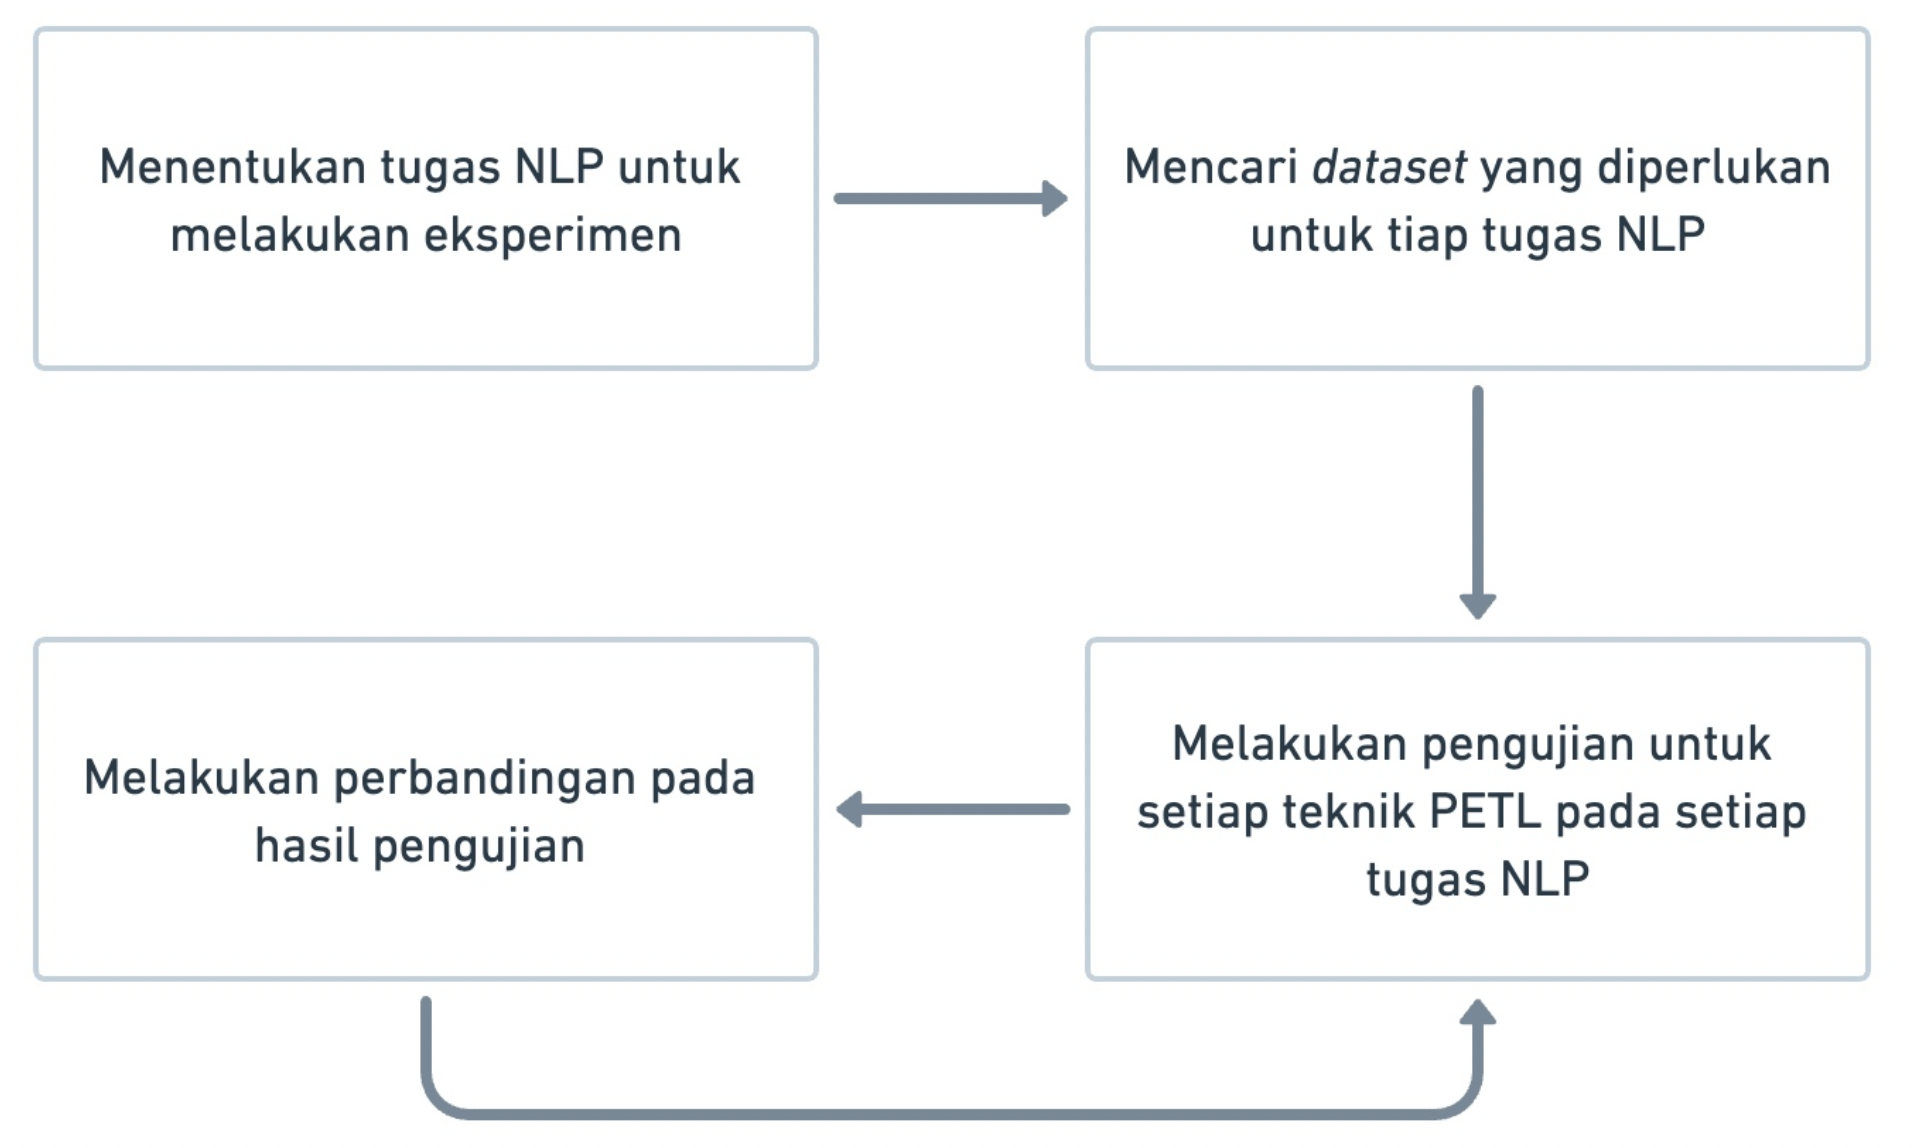
\includegraphics[width=0.8\textwidth]{chapter-3/langkah_umum.png}
    \caption{Langkah Umum Solusi}
    \label{fig:langkah-umum}
\end{figure}

Dataset yang diperlukan akan diambil dari \cite{nusacatalogue}. Teknik PETL yang digunakan adalah LoRA (\textit{Low-Rank Adaptation}), \textit{Prefix-Tuning}, dan \textit{Tiny-Attention Adapter}. Hasil pengujian berupa kinerja dari teknik PETL serta penggunaan sumber daya dari setiap eksperimen.